\documentclass[a4paper,11pt,twocolumn]{article}
\setlength{\columnsep}{0.5in}
\usepackage{url}
\usepackage[letterpaper,margin=0.75in]{geometry}
\usepackage{times}
\usepackage{graphicx}
\usepackage{listings}
\usepackage{color}

\definecolor{dkgreen}{rgb}{0,0.6,0}
\definecolor{gray}{rgb}{0.5,0.5,0.5}
\definecolor{mauve}{rgb}{0.58,0,0.82}
\usepackage {algorithm2e} 

\begin{document}

\tableofcontents

\title{SDN$^{2}$: Marketing System for Data-center Network Resource Allocation based on Software Defined Network}
\author{Rui Zhou \and Shu Zhang}
\date{Final Project - CSCI 2950-u - Spring 2013}
\maketitle

\begin{abstract}
In this report we present SDN$^{2}$, an auction-based Marketing \underline{S}ystem for \underline{D}atacenter \underline{N}etwork Resource Allocation based on \underline{S}oftware \underline{D}efined \underline{N}etworks.
Motivated by similar mechanism of auctions for resource allocation in other computer systems, we aim to 
let users bid their network resources. Currently our focus mainly lays in bandwidth and latency for desired flows. Different from the only   
bidding system for Network Resource existing in Google's Data-center\cite{google}, our system is based on Software Defined Network and takes the advantage
of the central controller and global network information. 
Another aspect of our focus is on the allocation algorithm for the auctioneer. We proposed and investigated some 
algorithms as well as evaluated the performances of some of them. 
\end{abstract}

\section{INTRODUCTION}
%resource allocation and network resource allocation in dcs
Resource allocation is an important topic in system related area, especially in data centers where resources distribution heavily influences the performance 
of the application running in the data-centers. Since the network resource is limited and application expense could be infinite, the idea of launching auctions on
data-centers for applications to bid resources comes to existence. With the core of auction, some marketing mechanisms have been built for public or 
private data-centers, such as AWS\cite{aws} or internal data-centers for large companies such as Google and Microsoft. While various types of marketing systems
emerges, they primarily focus on the allocation of computation power and storage room, few of them cares enough about network resources, let along combining with the existence of SDN network. 

%sdn
The emergence of SDN network   provides network manipulators with more powerful 
ways to manage their networks. For example, the existence of NIB(Network Information Base) in Onix\cite{onix} could provide the upper layer with the global
topology of the entire network just in a single manager machine.  SDN also provide the ability to configure the switches in the networks on the fly, thus a more dynamic way to bid and evolve the network could be built.

%this paper: an combination
In this paper we combine the idea of auction in data-centers networking with the SDN technology so as to reach the goal of bidding network resources. 
Since we have the central information of the network, bidding and allocations of requested resources could be performed in a single node in the network(aka. the controller) quickly to reach the goal of real-time allocation. The general work flow is shown in figure 1. 

\begin{figure}[ht!]
\centering
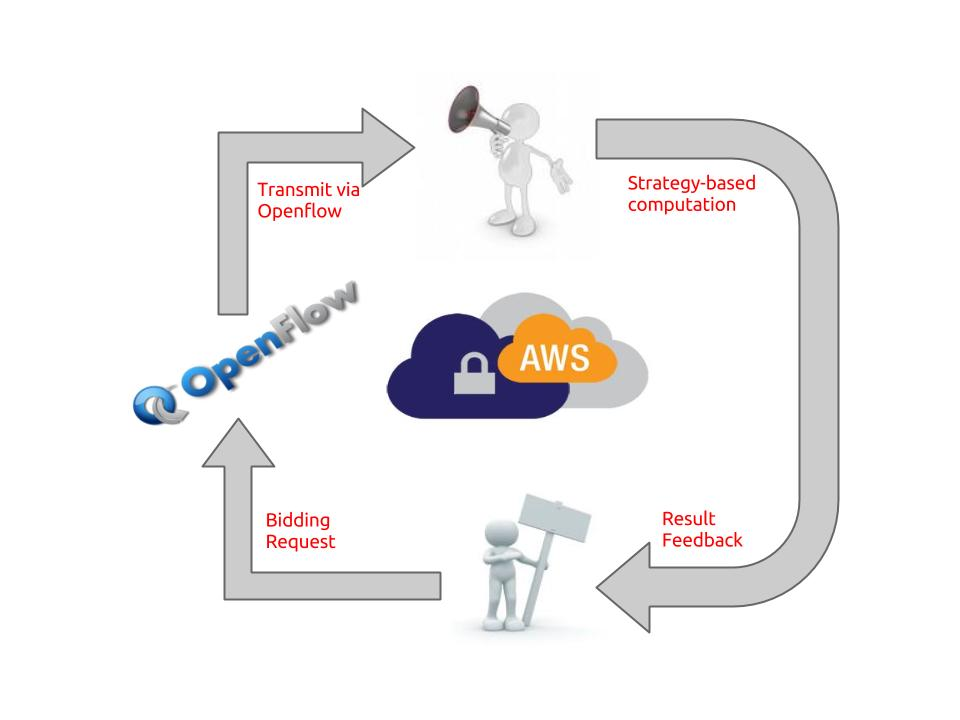
\includegraphics[width=90mm]{general_flow.jpg}
\caption{Auction Working Flow}
\label{overflow}
\end{figure}

% overall work flow
The general flow for each round of bidding starts from the bidders. Bidders first recognize their flow requirements in the near future, for example, they might need to reserve the resource for a flow 
from host A to host B in the network with a certain amount of data to transfer, with the hope of minimum bandwidth and latency (QoS) guarantees in 
a certain time period. After confirming these requirements, bidders send bidding requests to the auctioneer. The auctioneer collects requests for this 
round and wait for the bidding clock to go off, saying it is time to calculate the allocation. With specific allocation algorithm, the auctioneer could
get a Boolean result for each bidder's request and send the feedback to the bidders, and then a new round starts.

% goals
Our goals for this project are  to build a workable system running the auction and doing allocation in real time,  to provision a 
protocol (a standard interface) for all parties wishing to use the system to follow so as to communicate using the protocol, and  to investigate
algorithms to allocation resources basing on requests, for different goals. 

% sections
In section 2 we investigate some existing backgrounds that serves as inspiration or basement for this project. In sections 4 we conclude the contribution  of our work. 
In section 5 the design and algorithms of the system are discussed and in the implementation is introduced in section 6. In section 7 we do some 
experiments and evaluation on the out-coming products. Since our system is still in prototype, in section 7 we have identified some extensible
work which would be done in the future. And in section 8 we discuss some related work.


\section{KEYWORDS \& CATEGORIES}
Data-center, Network Resource Allocation, Marketing and Auction, Software Defined Network.



\section{BACKGROUND}
In this section, we investigate     existing data centers (mainly private data-centers and public data-centers) and their marketing and 
pricing models. Also, we introduce the existing techniques of SDN which is the base of our system.
\subsection{Data-center Markets}
There are generally two types of data centers, one is for-profit, public cloud data-centers, such as Amazon Web Services\cite{aws}, the other is private cloud
data-centers, like those operated by Google or Facebook. Although auction mechanisms could be applied to both, different scenarios results in diverse answers because of 
their business models.  Although most of the models applies in computation and storage marketing, they serve the same principle for our Network Allocation System.
% The following two paragraphs talks about the assumed behavior for the two types of data centers in this paper and our discussion are 
% based upon these behaviors.

In a public cloud service, bidders are customers who use the cloud service. Take Amazon EC2 for example\cite{ec2}, Amazon revises prices for instances for all kinds
of types. Three basic types are On-Demand Instances, Reserved Instances, which allows user to reserve a period of time for future uses and Spot Instances\cite{spot} whose values 
fluctuate and allow customers to bid on them. Along this path, Amazon created other services like data transfer, elastic IP addresses, elastic load balancing, etc and 
makes pricing policies for them. From Amazon's view, its pricing policies are so carefully revised so that they could maximize its profits. If a customer wants to bid for Amazon's 
resources, her knowledge is pretty limited, and Amazon hides the data center details from customers and only expose pricing history as hints for users to bid, and the budget
of buyers are real currency. 

In a private data-centers running inside IT companies, the customers are internal teams of companies who use the data-centers resources for the sake of their team and the companies.
The operator's goal might be minimizing the cost while meeting business objectives, or may be efficient use of network resources. The users (teams), according to their priorities,
are allocated different amounts of budget, which usually is virtual currency. Teams with more budget might use the data-centers resources in a higher share. The private data-centers 
might perform as a autonomy market, whose prices of goods are totally determined by the market or self-adapted by the system. Bidders, with higher possibility, will be
provided more detailed view of the data-centers conditions, such as dynamic traffic between servers or racks and static network topology, so that they could formulate their 
bidding policies more sensible. 
\subsection{Existing Pricing Mechanisms}
We found that the value of goods which are to be traded in the market is the core issue when letting a market run. People may argue that in an auction,
people could win the bidding by giving the highest amount of money per unit of resource. But sometimes it might be far more complex. Prices, in some cases,
are the reflection of the condition of the market, so it is better to set a baseline price for resources so that people who bid lower than that baseline will
never win the auction, even if they have the highest price. But in some cases, prices do not need  to be considered and the simple first-price or second-price auctions
policy could perform well. Also, complex cases like combinatorial pricing\cite{combinatorial auction} is also a must-to-think issue. Also, 
The pricing methods for auctions in private and public data-centers are pretty different. This is because the goals of markets in either data-centers are 
different. 
\subsubsection{Public Cloud Pricing}
Amazon\cite{aws} has set models for pricing in public cloud. AWS supports buy-at-once pricing for on-demand instances as well as auctions for resources
for spot instances. For on-demand services, prices for instances are relatively higher and the good thing is that they are guaranteed to be provided to the buers.
For Spot instances\cite{spot}, Amazon has set the base prices for instances. The prices are much lower (\$0.007 per hour versus \$0.060 per hour for on-demand instances).
The prices are given by Amazon according to their costs and virtual equipments with different capacities will have different prices. Resources
are provided in a combinatorial way, since it is meaningless to bid a single CPU without any memory or storage. But in some scenarios resources are not 
sold in a combinational way, such as Elastic Load Balancing which only charges by the amount of data to be processed by the load balancer.
\subsubsection{Private Cloud Pricing}
Unlike AWS, prices per unit of resources in the private cloud data-centers probably will change in a dynamic way.  Systems like D'Agents\cite{dartmouth} and Google's Planet-wide 
Clusters\cite{google} has adopted dynamic pricing and price of resources are updated periodically. Both the aforementioned systems uses dynamic prices to 
reflect the changing demand-supply relation. For dynamic pricing, the prices are the minimum payment. But in order to maximize the utility of total resources,
the sealed-bid second-price auctions \cite{second price} could be used so as to guarantee that as long as there are more than one bidders in a certain auction round, 
there will always be a winner. The dynamic minimum prices in this case, serve as an indication for bidders to price their bid requests. The prices in \cite{google} could 
change in an self-adaptive way. In short, 'hot' resources will be more expensive and a function (g(x,p)) calculates the price increment after each auction round, basing on the 
exceeding of demands over supplies. Interestingly, AuYoung, et al \cite{ucsd} discovered that auctions might take some time as bidder's patience falls down
when waiting for gaining the resource. So there should be another `buy-it-now' pricing mechanism provided for users who don't want to wait. The buy-it-now
pricing short-circuits the price discovery process of the auction, and the price is determined by a historical function which takes the historical auction/buy-it-now
prices for parameters.


\subsection{Software Defined Network}
\subsubsection{OpenFlow}
The very novel idea of Software Define Network was originally proposed by \cite{Greenberg_abstracta}. OpenFlow is one of the most popular and mature specifications for software defied network currently existing.  It is now   under actively development by the Stanford Openflow team and a very active  community.
OpenFlow primarily defines the control plane of the network. The core idea is that one or more central controllers are in charge of setting up forwarding rules in switches at the granularity of flows. A flow could be any set of packets that share some particular characteristics,i.e. source IP or destination port number. Packets matching a flow will be delivered by the switch according  to the flow rules, packets belongs to no flows will be forwarded to switches, The switches then will analyze the packet, determine the forwarding rules of this and similar packets.
OpenFlow does not require major changes to existing switches. Large portions of existing switches can support OpenFlow with proper firmware updates, and most of the switches vendors are now adding support for OpenFlow as a standard.
\subsubsection{Floodlight}
With OpenFlow as the foundation, several Openflow Controllers were deigned and implemented, including NOX, Nettle and Floodlight. Floodlight was originally developed by and has become one of most supported and widely used in both academia and industrial. Flooldlight is written in JAVA and highly Object Oriented.
Floodlight provides REST APIs for network administrator to take control of the network in the way OpenFlow provides. Meanwhile for developers, floodlight provides a plug and play fashion for them to 
add modules into the controller and add work flows. The controller side of SDN$^{2}$ system is implemented via the interfaces and rules Floodlight provides.


\section{CONTRIBUTION}
Our contribution are mainly building a marketing prototype over SDN and reaching some sort of marketing fairness by our allocating algorithm .
Also, our system could reach the performance requirement of real-time allocation, and supports further extension.
% what is new ?
%sdn
\subsection{Floodlight and SDN based}
Our work is mounted on Floodlight as its basement. With relatively mutual developed system, Flood light and
can be utilized in real world with few set ups thus make deployment of our project easier.


%fair on user/ flow / 
% resource utilization

\subsection{Marketing Fairness  }
Bob Briscoe in his paper\cite{bob} has bluntly pointed out that many fairness based on flows are pointless. He argues that
 flows are simply not the right
entities to provide fairness to. We believe in his argument, but it is also arguable that sometimes fairness over flows
can have its usages. 
% Algorithms such as max-min flow generally works well and many people are used to it. In our
% work, the total amount of virtual currency/cash  available in our market mechanism resource allocation system at a 
% particular time period is proportional to the existing resources available in that  particular period ,by the 
% factor of $\alpha$. The total currency/cash is equally distributed to end entities(users or flows) at the beginning of that
%  time period. This design will automatically generates fairness among all the users(or flows) and make sure the 
% total requests from the users unlikely will  burst too much and exceed the ability of the system. 
% The factor $\alpha$ can be 
% adjusted over time to reach the best utilization of available resources at each time period. The total traffic 
% in  our resource allocation system can be treated as one giant flow with large weight, thus min-max flow can be used
% among this  giant flow and others to achieve the maximum usage for all time over the entire system. Weights between users and flows can be 
% maintained by adjusting the distribution of virtual cash. Every user has equal amount of virtual cash in a evenly 
% weighted system and the properties of strategy-proof and envy free are automatically granted.
A great benefits that we obtain from utilizing auction based Network resource allocation is that the fairness issue is no longer so relevant. It is up to the user to reserve and use the network resources. The Auctioneer treats everyone equally as they all have to bid.



%speed -> search
\subsection{Solve Fast}
Different from allocation for computing resources, the allocation for Network resources requires a much high 
decision speed. In \cite{Sai}, Sai proposed the pattern for agents to keep bidding and potentially face the failure. This works in computation and storage allocation but is
probably not the best strategy in the design of our system. 
% In our work, we had a close look at ideas in logical programming
% and tries to seize the best out of it. Our system primarily operates as tree search in a solution space composed
% with users' bids are our search are target to optimize a ``profit'' of certain kinds. There isn't much bidding failures
% in our system. The amount of virtual cash a bidder spends mainly affect the priority of their resource allocation. 
In our work, other than the adjustable time needed to gather the requests for a bidding round, our controller can choose to utilize algorithms and strategies that compute fast and obtain a solution that may not be optimal but good enough. The Income-Utilization Strategy we implemented is  $o(nlogn)$ in time complexity and linear in space thus can produce allocation really fast. Some of the computation such as latency validation of requests can even be done in parallel while the system is gathering bids. Thus we argue that given proper strategies, our system is scalable and fast.
% In our observation, the major delay before the bidder could use the network would be the time needed 


\subsection{Extendable Strategies}
Strategies are nothing special but plug-gable modules that can be switched immediately. Although few strategies have been implemented,  
Our system could potentially support multiple optimizing modes including : ``Short job first''. ``Maximun profits'', ``best utilization'',
``most met deadlines'' and so on. It is up to the system manager to decide what to use.


\section{SYSTEM DESIGN AND ALGORITHMS}

\subsection{Pre-Assumption}
In order to let the system work, we have some pre-assumptions so as to limit the environment. First, we don't specify the unit of 
currency. Although in practice the type of currency should be figured out whether real or artificial, in this system prototype we assumed
the we present money as a LONG type of value. Secondly, we don't care about where and how users gain their money they use to bid. Although in
some existing systems like \cite{ucsd}, all bidders are allocated money at first and then their wealth are adjusted by the bank profit and 
social welfare mechanism, our scenario does not have an `invisible hand` which proforms as a government. Thirdly, our system only works on 
networks with full deployment of SDN networks. Currently the sysetm does not support networks with multiple islands, some of which are 
OpenFlow enabled while others are not. Fourthly, we only constrain users to bid for the machine they reside. 
So if a user in using a machine, he could only bid for flows starting from the using machine. Although supporting
users to bid for other machines are not hard to achieve, we just want to limit the rights the bidders could hold in the network. Another thing 
is that the bidder coud only bid for the future. If it bids for the past, the time will be invalid.
The final major assumption we make is that the working controller never goes down. Since we store 
information in main memory, if the controller crashes, all bidding information maintained in the bidder will be lost, and without the 
replication mechanism it will be a huge problem in our system. For now we temporarily put aside this consideration, and we plan to add
the fail-over mechanism in the future. 



\subsection{Design and Architecture}
In this section we introduce the design and architecture of our system,
%  and also points out our solution to the cafeterias. Also, 
we rule a protocol of exchanging bidding messages which runs in the application layer. There are two major  components of the system,
one is running inside the Floodlight controller, which acts as the auctioneer and the other is running on the client machine, 
which performs as a bidding agent for the client. These two sides communicate using the bidding protocol. 

\begin{figure}[ht!]
\centering
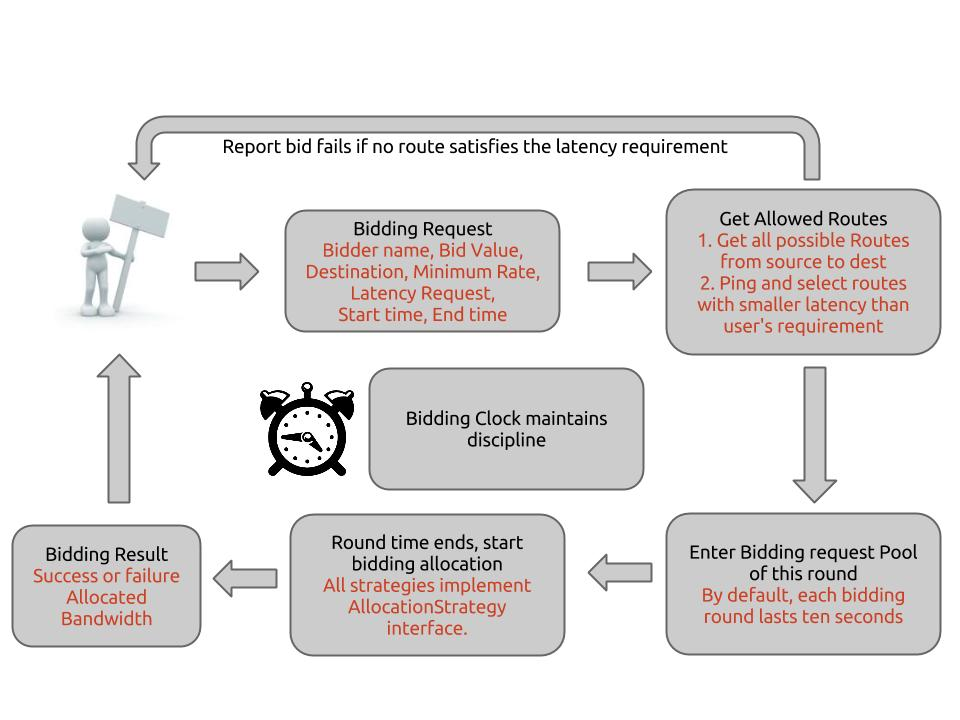
\includegraphics[width=90mm]{flow.jpg}
\caption{Bidder-Auctioneer Interaction}
\label{overflow}
\end{figure}
The interaction between bidders and auctioneers is shown in Figure 2. The bidder sends a bidding request in each round, currently, the 
system needs the user to fill in required fields, including his name, his bidding value, the destination of the flow he wants to bid,
the minimum transform rate he accepts (in the unit of MB/s), the latency he accepts for a packet to 
travel from the source to the destination and the start and end time of the transmission. If 
some fields are what the bidder does not care about, for example the latency, he could just set a special value such as Float.MAX\_VALUE to that field. But 
the start and end time must be set because the computation requires these two fields to be definitely set. Then the bidding request is set 
to the auctioneer (aka. the bidding manager). Whenever the bidding manager gets a bidding request, it immediately verifies whether the latency
could be satisfied. Because the bidding manager resides in the Floodlight controller with the global topology view of the network, so it could
get all possible routes using the source and destination node. Then for all possible routes, it sends probe packets and count for the time the 
packets use to pass all routes. The administrator could set how many times probe packets are sent for each verification in order to get an 
average real-time latency for the route, or the minimum if we are being rigid. If the users' required latency is smaller than the actual probed latency, we just send an bidding 
feedback to the client saying the bid could not be satisfied because of the latency issue. Then for each bidding request, if one of its possible
path could satisfy the latency requirement, these verified routes, along with the original bidding information, are packed together to get into
the bidding request pool, waiting for the bidding round to come. Then for a certain period of time, the auction time arrives, all bidding requests
in the pool are collected and calculated for their results. Then the results are sent to the bidders, which marks the end of the round.

A special feature of our system is that we never over saturate any links. This means we simply do not allocate more than the network can accept, at the granularity of each switch port. The bidders can have to send the packets through a rate limiting box either in their bidding system or implemented as rules in the first switch that connected to that host. Given this design, it is nature that the latency will be overall consistent regardless of the actual traffic load. While this design also requests the strategies to be smarter to allocate more while avoid saturate the bottle neck.

\begin{figure}[ht!]
\centering
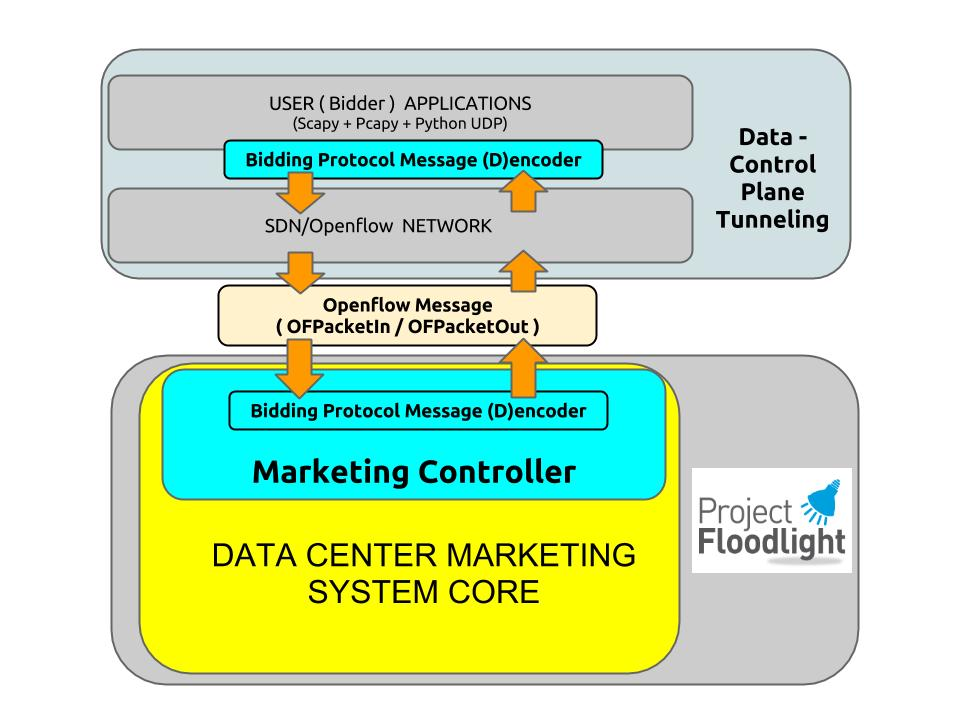
\includegraphics[width=90mm]{architecture_controller.jpg}
\caption{System Architecture}
\label{overflow}
\end{figure}

The system architecture is shown in Figure 3. The user side sends and receives bidding messages formatting in the bidding protocol. These
messages are transmitted via the SDN network. As there is no control plane links from hosts to the controller. The packets are sent in the data plane to the switches, destined to the controller which resides
in the control plane. We utilize the feature of OpenFlow that if the switch does not know the destination IP of a packet or it has not a rule
matching the head of the packet, the swtich will transfer the packet to the controller as a PACKET\_IN message, hence letting the packet go into
the control plane. So the marketing controller is listening the packets as a module of the floodlight framework. If it gets a packet from a 
special IP we make as a mark for the bidding message, the Marketing Controller will decode the message and packet it into a bidding request 
object and pass it to the Marketing Manager which lays in to logic layer, then the Manager could do the thing described in the last paragraph.


\subsubsection{The Bidding Protocol}
There are generally four types of packets we use to pass mesages between bidders and auctioneer. In a typical data-centers, we assume the IP addresses 
are highly clustered and irregular IPs does not appear. So first we assigns speicial IPs for the bidding protocol packets so that either side could 
recoginze the special packets in the data plane. Then we serialize the packet informaiton in JSON. The reason we use JSON is that we want the protocol to
be acoomodated to various machine and data presentation types. 

The bidding request packet is used for the bidders to send their requests to the auctioneer. The bidder name is a String type in Java, and other 
values are all Long (32 bits). Since we only allows users to bid 
for a future period of time, the Start and End time fields in the packet must be positive values and they 
are presented as the relative offset of time comparing with the current time (presented as a long value in the central controller and
we assume the user could know the current time). The speicial source IP for the bidding request packet is 1.2.3.4. The bidding result packet is sent by the auctioneer to the 
bidders. The speicial source IP is 1.2.3.4 and the bidding result is a boolean type and the allowed rate is a allocated rate which must be no smaller than the 
user's requested rate. The latency probe packet is used for the controller to probe the real-time latency between two nodes. The source and destination IP
are set by the controller as the real IP of the two nodes (before sending the latency probe packets, the controller should establish rules on all
switches on the path, using the two IP as matching fields, the out port for the last swtich is 6632 which directs the packet back to the controller).
The Send Reminder Packet is used for reminding bidders to send their flows when their winning bidding time comes. The speicial source IP is 1.2.3.5. The 
packet tells the controller where is the destination of the flow and the duration of this transmission. The reminding mechanism is facilited by the 
timers so that the bidders don't need to record what they have won. The Marketing Manager records these information for the bidder and when the start time 
of their winning bids arrives, the reminder packet is sent. When the bidder receives the reminder packet, it will start sending UDP/TCP packets. The 
bidder does not need to set the route and rate limiters because the controller has already set the rules in switches on the route and set a rate 
limiter on one queue of the first swtich of the flow's path.

\begin{figure}[ht!]
\centering
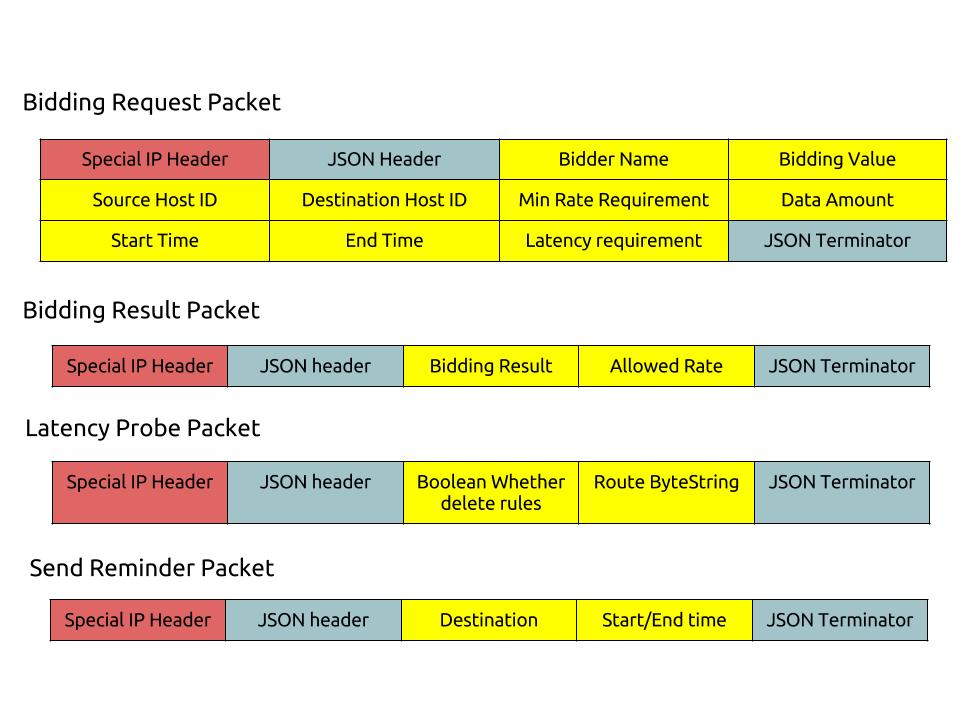
\includegraphics[width=90mm]{protocol.jpg}
\caption{The bidding protocol}
\label{overflow}
\end{figure}

\subsubsection{Marketing Manager}

\begin{figure}[ht!]
\centering
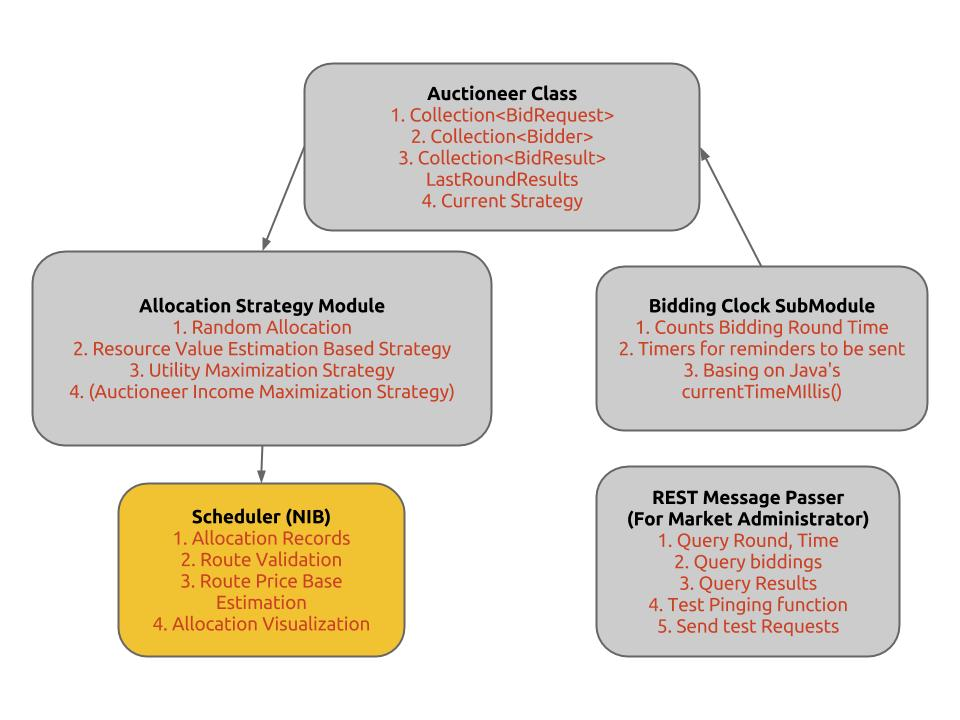
\includegraphics[width=90mm]{core.jpg}
\caption{The Marketing Manager (Auctioneer) Modules}
\label{overflow}
\end{figure}

The internal modules of the Marketing Manager is shown in Figure 5. The marketing manager receives and sends bidding related objects passed by 
or to the lower level bidding controller. The Auctionner object is a singleton, which maintains all bidding requests of this round (it also
has a list of coming bidding requests of next round in case it is calculating the allocation for this round but some bidders have started
bidding for the next round), the information of all bidders who have participated in the bidding from the start, and the results of last round.
It also maintains the current allocation strategy. The bidding clock is in pace of the real world time. It sends a signal every 10 seconds (the 
bidding cycle time we set) to the auctioneer to perform an auction calculation. In the allocation strategy module we provide three strategies,
one is first-come-first-serve random allocation, the second is the resource value estimation based strategy, which is also called Income and Utilization 
Index based strategy, and the third is a mutation of the previous one, which aims to maximize the utilization of bandwidth resource. A rather
important part is the Scheduler module, which serves as our Network Informantion Base. The Scheduler is responsible for record all historic 
allocations (mainly their starting and ending time, their routes and their sending rate). The scheduler provides an interface for allocation methods
to verify whether an bidding request is valid in that certain time period by doing the checking using its recorded information. Lastly, the Marketing
Manager holds a seperate module for system administrators to use REST APIs to set and test some functionalities.

\subsubsection{User side bidding agent}
As long as the potential bidders could follow the bidding protocol, they could build their client bidding program (the bidding agent) in any language
in any form. But there ar some hints for buiding the bidding agent. One is the bidders have to listen to potential incoming packets and analyze 
their IP address to see whether they are bidding messages. Another is that the user has to construct the bidding packet by himself, so he could 
manipulate all fields of the packet. 

\subsection{Auction Strategies}

In our system, the marketing manager can utilize different strategies to selectively satisfy the bidding requests. The bidding strategies are essentially moduli-zed parts that can be easily selected and loaded. In this section we talk about several related strategies.

\subsubsection{Implemented Strategies}

We have successfully implemented three strategies: first come and first serve, income and utilization index(formally called estimated index), 
and utilization index. Our evaluation shows that our income and utilization index can achieve significant better performance regarding the
 combination utilization and income comparing to the very natural first come first serve model which is sort of the standard naive philosophy 
to allocate network resources. Here is the algorithm we developed to provide the income-utilization index of a given route: 

\providecommand{\SetAlgoLined}{\SetLine}
\providecommand{\DontPrintSemicolon}{\dontprintsemicolon}
\vspace{5mm}
\begin{algorithm}[H]
\caption{Income-Utilization Index Calculation}

\SetAlgoLined
 \KwData{Desired Allocation alloc which contains the bandwidth information, Route rt, which is essentially a collection of switch ports}
 \KwResult{Income-utilization Index of  rt}
 price=0\;
 \For{each switch port p in rt}{
  bandwitdthPrice= alloc.bandwidth/p.leftOverBandwidth\;
  queuePrice= 1/p.numOfLeftOverQueues\;
  \eIf{bandwidthPrice$>$queuePrice}{
   price+=bandwidthPrice\;
   }{
   price+=queuePrice\;
  }
 }
  index=alloc.moneyWillingToPay/price\;
return index\;
\end{algorithm}

Each routes in collected in a bidding round thus is indexed and sorted, we then go over the list from highest index to lowest index, trying to satisfy as many routes as we can in that order.
Although no formal mathematical proof is provided, we take the  intuition that this approach encourages users to bid for the less contingent areas of the network at a granularity of switch ports, but also allows user to pay more and make reservation on bottleneck links. Our later evaluation section will show that this algorithms works well in practice.

If we change the  molecular in the equation of computing the Income-Utilization Index to 1, we have eliminated the affect of users' bidding price thus only focus on encouraging balanced utilization of the entire network. This strategy is indeed our utilization index implementation, which was also  tested by us. However we do not provide more discussion around this approach other than the information that in our test, solo utilization index not only fails obviously  in cumulative income but also sometimes fails in optimizing overall utilization of the network. The exact reason remains un-investigated, but we argue that it may perform better in bigger topologies with more bottle links than our test topologies.

\subsubsection{Envisioned Strategies}
We have some envisioned strategies that we did not have the time to implemented, 
one of them is indeed seeking for the optimal income in a strict way, some packages like SuanShu and CPLEX 
could help we put it into code into near future, the algorithm is decribed as following :

\providecommand{\SetAlgoLined}{\SetLine}
\providecommand{\DontPrintSemicolon}{\dontprintsemicolon}
\vspace{5mm}
\begin{algorithm}[H]

% \DontPrintSemicolon
\SetAlgoLined
 \KwData{Bidding requests received for a typical auction round, presented by a vector R:
 $$( R_{1} ,R_{2} ,R_{3},...,R_{n} )$$}
 \KwResult{A corresponding vector with each member a binary value indicating for each bidding request 
whether or not to accept their requests. Presented as: $$(x_{1}, x_{2}, x_{3}, ...,x_{n})$$ }
 \end{algorithm}
\begin{algorithm}[H]
 \For{each request in the request vector}{
    rank request by their starting time, get the modified reqeust vector R':
     $$( R_{1'} ,R_{2'} ,R_{3'},...,R_{n'} )$$
 }
 \end{algorithm}


\begin{algorithm}[H]
\caption{Imcome Optimization Algorithm}
 Create G as the container is used to store all requests with overlapped request time period \\

 \For{each request r in R'}{
  \For{each request r' in requests other than r in R'}{
    \If{ r'.startTime $<$ r.endTime}{
     group r' into r's time intersection group g
    }
  }
  add g into G
 }

 create a container G' for grouping requests intersected with switch-port pair in their sharing time period \\
 \For{each group g in G}{
  \For{each request r in g}{
   \For{ each switch-port pair sp in the route of r }{
    \eIf{ sp's group is in G' }{
      add r into the sp's group
    }{
      create sp's group in G' for this time period, add r
    }
   }
  }
 }
 
 Initialize the result vector RV, \\
 Set up the optimization goal, which is to maximize:\\
  $$ V((x_{1}, x_{2}, x_{3}, ...,x_{n}) = \sum_{i=1}^{n} x_{i} * R_{i}.value$$
 
 Set up the constrans : \\
 \For{each switch-port pair sp in each g' in G'}{
   $$ \sum_{i=1}^{n} x_{i'} * R_{i'}.min_bandwidth < sp.remainRate $$
 }
 
\end{algorithm}



%sigh .... the following is not achieved

% \subsection{Criteria of the System}
% % requirements from five star paper
% In [Dominant Resource Fairness: Fair Allocation of Multiple Resource Types], Ali Ghodsi et al'\cite{ali} discussed Dominant Resource Fairness towards 
% Fair Allocation of Multiple Resource Types regarding the computation and storage resources. In their discussion several cafeterias
% are used to judge one allocation strategy. In this paper, we will adopt the cafeterias but treat the word  word ``cluster'' as ``Network resources'':
% 
% \begin{description}
% 
% \item 
% [Sharing Incentive:]
% Each user should be better off
% sharing the cluster, than exclusively using her own
% partition of the cluster. Consider a cluster with identical nodes and n users. Then a user should not be
% able to allocate more tasks in a cluster partition consisting of $\frac{1}{n}$ of all resources.
% 
% \item 
% [Strategy-proofness:]
% Users should not be able to
% benefit by lying about their resource demands. This
% provides incentive compatibility, as a user cannot
% improve her allocation by lying.
% 
% \item 
% [Envy freeness:]
% A user should not prefer the allocation of another user. This property embodies the
% notion of fairness [13, 30].
% 
% \item 
% [Pareto efficiency:]
% It should not be possible to increase the allocation of a user without decreasing
% the allocation of at least another user. This property is important as it leads to maximizing system
% utilization subject to satisfying the other properties.
% 
% \end{description}
% 
% 
% and In addition  four
% other nice-to-have properties:
% 
% \begin{description}
% 
% \item 
% [Single resource fairness:] 
% For a single resource, the
% solution should reduce to max-min fairness.
% \item 
% [Bottleneck fairness:]
%  If there is one resource that is
% percent-wise demanded most of by every user, then
% the solution should reduce to max-min fairness for
% that resource.
% \item 
% [Population monotonicity:]
% When a user leaves the
% system and relinquishes her resources, none of the
% allocations of the remaining users should decrease.
% \item 
% [Resource monotonicity:]
% If more resources are added
% to the system, none of the.
% \end{description}
% 
% DRF are able to provide all of the above except for the last \textbf{Resource Monotonicity}.
% In fact Ali Ghodsi et al' also gives the follow theorem:
% \newtheorem{thm}{Theorem}
% \begin{thm}
%  No allocation policy that satisfies the sharing incentive and Pareto efficiency properties can also
% satisfy resource monotonicity.
% \end{thm}
% 
% In this paper, we will show that our work can satisfy no less than DRF. In fact, because of the design of our work, several of 
% those properties are guaranteed without the need for special care and we can   potentially tackles all of the
% properties by in several particular scenarios, which the theorem may not apply due to the design level advantage of our work.



\section{IMPLEMENTATION DETAILS}
Our prototype system is consisted of two programs, one resides in the FloodLight and another is the bidding agent we build in Python. There are roughly 
6000 lines of Java code and 500 lines of Python code. The low level marketing controller is a Floodlight Listener listening for any PACKET\_IN messages.
In order to let our special bidding packet with special IP to be transferred to the listener, we modified the floodlight controller (implementation 
of IFloodlightProvider) to let it not filter out the bidding mesasge packets. The route is presented by the Floodlight as a list of switch-port pairs,
and Floodlight provides an interface to list all possible routes between any two switches, so an additional hashmap should be used to recordthe host machiens
and their attachment points. In the client side, we use scapy to construct packets and forcely push them into the ethernet, so as to ensure the packet 
could be pushed to the attached switch. Then we use pcapy to sniff all packets coming and select packets with IP address 1.2.3.4 or 1.2.3.5. There are mainly
two threads, one is for sending bidding requests and the other is listening to the coming packets in UDP. 


\section{EVALUATION}
We have tested the performance with the aid of Mininet\cite{mininet}. 
We have primarily tested First Come First Serve, Income and Utilization Index over three 
different topologies for more than 20 bidding rounds each.  As an overview, 
our Income-Utilization index helps to achieve similar or a little better overall utilization, 
while achieves significant better income/utilization rate. Figures 6-14 show the details.

\begin{figure}[ht!]
\centering
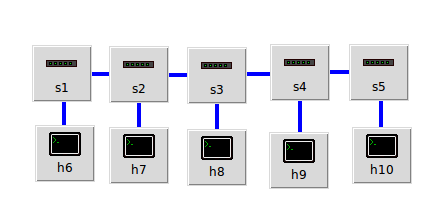
\includegraphics[width=70mm]{line.png}
\caption{Line Topology}
``Mr. LAN''
\label{overflow}
\end{figure}


\begin{figure}[ht!]
\centering
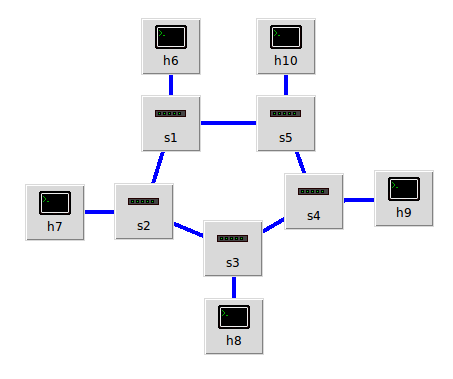
\includegraphics[width=70mm]{circle.png}
\caption{Circle Topology}
``The Ring''
\label{overflow}
\end{figure}


\begin{figure}[ht!]
\centering
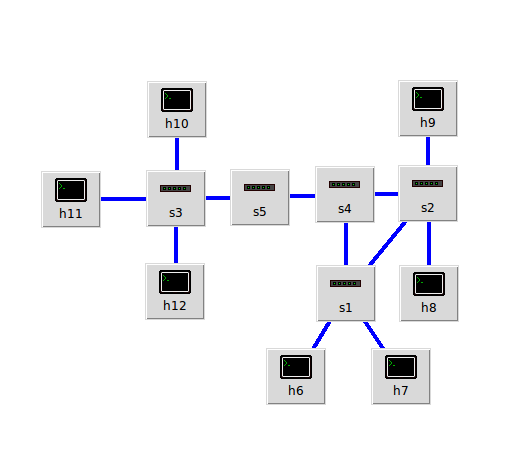
\includegraphics[width=80mm]{mytopo.png}
\caption{Complex Topology}
We call it complex because it contains a circle and a line.
\label{overflow}
\end{figure}

\begin{figure}[ht!]
\centering
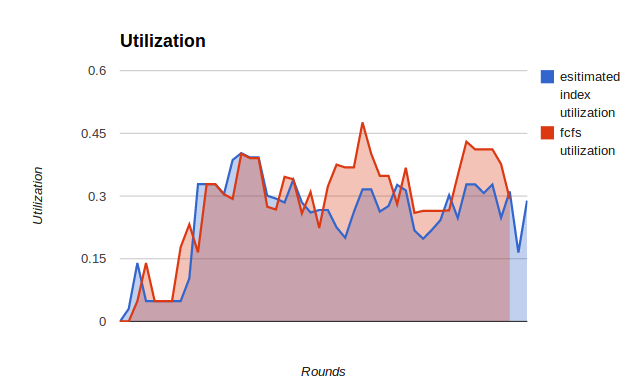
\includegraphics[width=90mm]{circle_utilization.png}
\caption{The utilization comparison in circle topology}
\label{overflow}
\end{figure}

\begin{figure}[ht!]
\centering
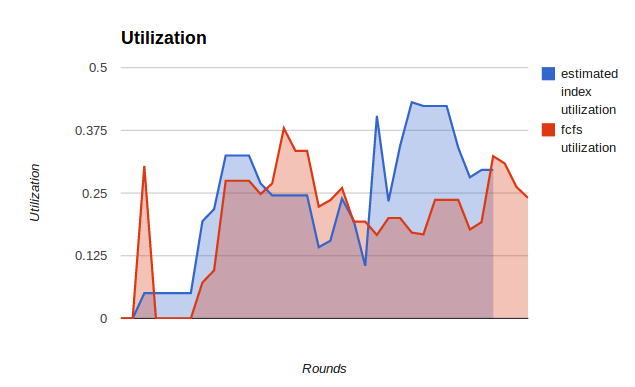
\includegraphics[width=90mm]{line_utilization.png}
\caption{The utilization comparison in line topology}
\label{overflow}
\end{figure}

\begin{figure}[ht!]
\centering
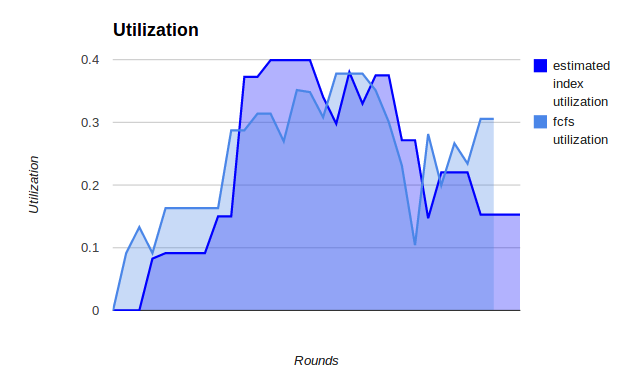
\includegraphics[width=90mm]{mytopo_utilization.png}
\caption{The utilization comparison in complex topology}
The aggressiveness of FCFS is very obvious, and FCFS appreantly does not do well regarding the long run.
\label{overflow}
\end{figure}

\begin{figure}[ht!]
\centering
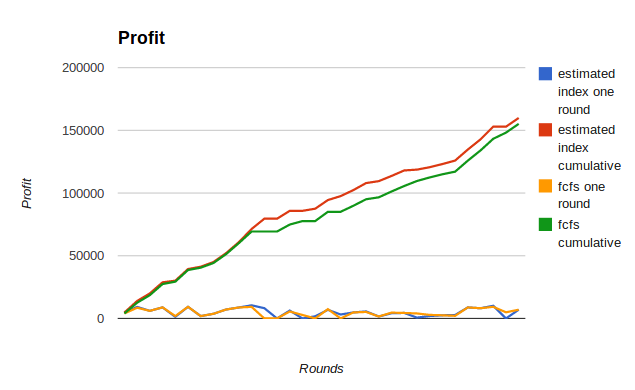
\includegraphics[width=90mm]{line_profit.png}
\caption{The profit (income) comparison in line topology}
The lines crawling underneath are for income per round.
\label{overflow}
\end{figure}

\begin{figure}[ht!]
\centering
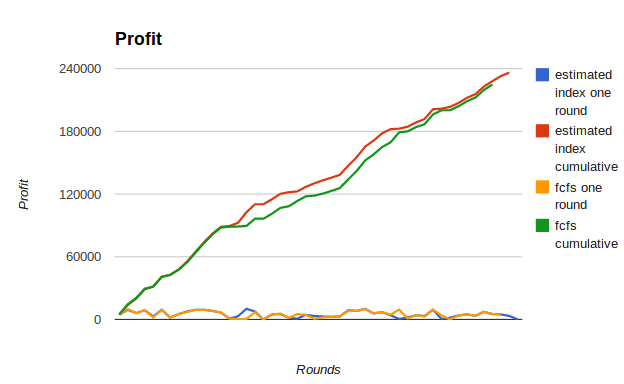
\includegraphics[width=90mm]{circle_profit.png}
\caption{The profit (income) comparison in circle topology}
The lines crawling underneath are for income per round.
\label{overflow}
\end{figure}

\begin{figure}[ht!]
\centering
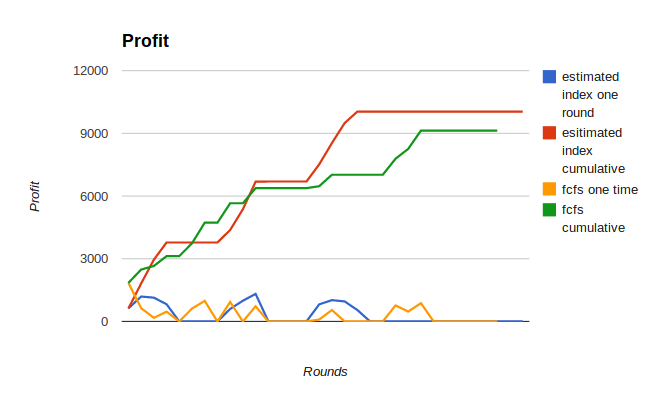
\includegraphics[width=90mm]{mytop_profit.png}
\caption{The profit (income) comparison in complex topology}
The lines crawling underneath are for income per round.
\label{overflow}
\end{figure}

\section{DISCUSSION AND FUTURE WORK}

Our system is a good starting prototype, the novel idea was there but lots of potential components are remaining to be 
further developed and researched. Some particular interesting potential future work including :

\subsection{Stability Issues}
A significant unsatisfactory we have so far is the stability issue when we test on our Mininet testbed. 
The stability issues happens in multiple forms.  One clear understood common reason the system fails is when the user 
started to bid before the internal controller configure everything it needs. The coming in bidding packet could result in
 exceptions in various place of the system, depending the stage the system is currently within intiliazation phase. 
Besides the obvious easy to fix issues, we sometimes experience random time out of virtual switches simulated by mininet. 
A very common issue is that, floodlight controller would suddenly timeout the netty channel through which a switch is connected, 
due to read time out. Almost instantly after the switch was timed out and disconnected, the controller will detect a new switch 
in mininet, with different real machine port number. This issue happens occasionally, its reason is unknown yet and could resides
 in at least one of floodlight, netty framwork, mininet  or the reference swicth implementation.

\subsection{More Tests and immigrate to real world test bed}
Because of the limit of time and the delay caused by bugs hard to trace(ie, the switch loss bug mentioned aforehead), 
we did not have time to test our system with real switches. It is definitely an item into our todo list and needs to be done in the future.

\subsection{Support of Partial Bidding Request}
In our current settings, users can make request without any requirements on Latency. The user could simply indicate that the latency 
is not important and the bidding agent  could translate as and Long.MAX\_VALUE to put into the request message. However,
 we have not provided a standard when the client only have request for latency but not bandwidth. As a bandwidth of zero make
 no sense regardless of its associated latency, this problem may further redirected to be to help user determine their needs for bandwidth.

\subsection{ Request Translation}
Another very realistic request from users may be the following. 
Most of the users are not able to provide an information detailed enough to assemble a bid request for our system. 
For example, user Bob may only want to download this one Gigabtyte movie tonight so he could watch it tomorrow, 
thus the latency is not so relevant and the shape of his allocation is elastic and dividable. Or 
Alice may want to schedule a phone call  after five minutes and does not really want to specify an end time for it, 
as she does not know in advance. Her request might be composed of an minimun latency, an minimum bandwidth in an extendable session. 
All those real world requests need to be translated by our bidding agent to fits in our bidding system, and our bidding system
 could extend its rules to fit more complex and realistic scenarios. 

\subsection{ Request Predication}
Yet the biggest gap between our system to widely pratical usage is that most of the regular users may not want to make a bid, 
either not able to or no bother to. Thus a great break through that will benefit our system greatly would be enable our bidding
 agent to bid for the users by predicting the potential requests.  Prediction of user requests is solo a much harder problem that 
people are trying to tackle(example ref paper), and its advance could benefit not only our data-centers marketing system but also many 
other existing systems. But as aforementioned, it is generally very hard to achieve in current state of art.



\section{RELATED WORK AND COMPARISON}
Data-centers have rapidly evolved to become the dominating server style in almost
any modern Internet based organizations. As the amount of computation and associated
network  traffic keeps increasing, the needs for efficient and fair  allocation in  Network resources
has also becomes a important topic. There exist enormous number of devices with all 
kinds of different hardware and software among all the data-centers. Different processes and users could
have different requests and requirements. A Hadoop cluster running Map-reduce computations 
may requires great bandwidth.
A web search engine clusters such as Google may want to response to a request 
within a relatively rapid time. All of the needs are to be solved with appropriate network resources
allocation.

% enormous number  of papers have discussed the resource allocation in clusters,
% regarding the computation resource, few on NETwork 
Allocating \textbf{computing and storage} resources such as Cpus and Memory
 in clusters and date-centers has been a popular topic widely discussed. Researchers have proposed and implemented
various algorithms to achieve fairness and efficiency among different entities. 
%{eaxmple papers} 
Rajkumar Buyya el at' \cite{Rajkumar} proposed architecture for market-oriented allocation of 
resources within Clouds that encompass both customer-driven service management 
and computational risk management to sustain SLA-oriented resource allocation. 

Artur   Czumaj el at'\cite{Artur} proposed  the first thorough theoretical study of the
price of selfish routing in server farms for general cost function, giving the hypothesis that 
distributed entities in data-centers are selfishly motivated.  
Ali Ghodsi el at\cite{Ali} presented fair allocation regarding dominant resources of multiple types
in a data center clusters.
Sai Rahul Reddy P\cite{Sai} in his Master's thesis proposed combined time and budget optimized auction 
algorithms in grid computing. 

However, there exists very few research focusing on the allocation
of \textbf{network} resources. We believe the allocation on \textbf{network} resources such as guaranteed bandwidth and 
latency are as important as the allocation of computing and memory resources. Computation and storage are not free
thus are entitled to allocation based on market mechanism, so is network resources. This is actually intuitive 
and commonly accepted patterns in real life. Phone carries would sell you a phone for very cheap price and make 
benefits from cellular services, this is a typical example in which the importance of allocation of network resource
 exceed allocation of computation and storage. In data centers, inappropriate abusing of network resources can results
in the failure of the whole system. It has noticed by network administrators that naively running TCP
between hosts can leads to huge overhead on lost packets. Domain specific algorithms like DCTCP\cite{Mohammad} are proposed and applied
in data-centers to effectively avoid collapse and keep traffic moving. But a more agile control was still very hard
to reach due to the distributed nature of inter connected systems, which lacks of a central controller with
a overview for the entire network and the needs of each entities are not really be collected and analyzed to form a strategy. The entire network also do not seek to optimize anything in general.
It would be great if we can have a central view of the network which contact with each participating hosts in the network and allocate resources to them efficiently. Note that
allocation of network resources often requires orders of  magnitude faster than allocation resources in Map-reduce style 
systems due to the fast nature of network transmission.  Thus regarding the allocation resource type, our system is very different but necessary.    


% software defined network and participatory network , a central view and participants
While the data-centers technology evolves rapidly, \textbf{Software Defined Network (SDN)} has also been proposed as a
stunning idea. By separating the control panel and the data panel, SDN   abstracts a supported network to be a networking system, which
offers a central view of the networks as a graph and provides a central controller based on flows.
Openflow is a dominating protocol used in SDN based Network systems which defines what is analog to the lower level API in an operating systems.
And high level Networking systems  such as NOX\cite{nox} and Floodlight\cite{floodlight}, and Nettle\cite{nettle} have been developed based on Openflow. SDN and
Network systems has been actively developed in many universities. Companies such as Big Switch and JUNIPER have long 
started to build SDN supported switches. It is believed that the future of network belongs to SDN. in this paper, we also take SDN as the approach towards the effective allocation of Network resources in data-centers. Recently Andrew et al' proposed 	\textbf{Participatory Networking(PNAE)}\cite{andrew}, 
which focuses on the collection of participating entities.  Pane provides serves    analog to the system calls to networking systems, which 
allow the  participating entities to provides hints to network systems and make changes to benefit their needs within allowed privileges.
PANE' structure  nicely forms the base of our allocation mechanism.  None of the  systems aforementioned utilize a central view of the network, thus we argue that our approach comes with naturally more potential. In  fact, only our system supports seamless switch between strategies and this feature comes naturally with the sets up. 

\section{CONCLUSION}

This project is so awesome, shu and ray are so great, please give us A. thanks. Just kidding.

\section{ACKNOWLEDGMENT}
Thanks Andrew Forguson and Rodrigo Fonseca. Special thanks to silao, who ate my sushi.



 


\begin{thebibliography}{99}
  \bibliographystyle{unsrt} 

 \bibitem{aws} http://aws.amazon.com.
 \bibitem{floodlight} http://www.projectfloodlight.org/floodlight.
 \bibitem{ec2} http://aws.amazon.com/ec2/pricing.
 \bibitem{spot} http://aws.amazon.com/ec2/spot-instances.
 \bibitem{mininet} http://mininet.org.
 \bibitem{Greenberg_abstracta}Albert Greenberg and Gisli Hjalmtysson and David A. Maltz and Andy Myers and Jennifer Rexford and Geoffrey Xie and Hong Yan and Jibin Zhan and Hui Zhang,
     ``ABSTRACT A Clean Slate 4D Approach to Network Control and Management''
 \bibitem{onix} Koponen, Teemu, et al. "Onix: a distributed control platform for large-scale production networks." Proceedings of the 9th USENIX conference on Operating systems design and implementation. USENIX Association, 2010.
 \bibitem{openflow} McKeown, Nick, et al. "OpenFlow: enabling innovation in campus networks." ACM SIGCOMM Computer Communication Review 38.2 (2008): 69-74.
 \bibitem{google} Stokely, Murray, et al. "Using a market economy to provision compute resources across planet-wide clusters." Parallel \& Distributed Processing, 2009. IPDPS 2009. IEEE International Symposium on. IEEE, 2009.
 \bibitem{combinatorial auction} Nisan, Noam. "Bidding and allocation in combinatorial auctions." Proceedings of the 2nd ACM conference on Electronic commerce. ACM, 2000.
 \bibitem{ucsd} AuYoung, Alvin, et al. Practical market-based resource allocation. University of California, San Diego, 2010.
 \bibitem{dartmouth} Bredin, Jonathan, David Kotz, and Daniela Rus. "Market-based resource control for mobile agents." Proceedings of the second international conference on Autonomous agents. ACM, 1998.
 \bibitem{second price} Vickrey, William. "Counterspeculation, auctions, and competitive sealed tenders." The Journal of finance 16.1 (1961): 8-37.
 \bibitem{clock1} Ausubel, Lawrence M., and Peter Cramton. "Auctioning many divisible goods." Journal of the European Economic Association 2.23 (2004): 480-493.
 \bibitem{clock2} Cramton, Peter, and Lawrence M. Ausubel. "The clock-proxy auction: A practical combinatorial auction design." (2006): 115-138.
 \bibitem{Rajkumar} Buyya, Rajkumar, Chee Shin Yeo, and Srikumar Venugopal. "Market-oriented cloud computing: Vision, hype, and reality for delivering it services as computing utilities." High Performance Computing and Communications, 2008. HPCC'08. 10th IEEE International Conference on. Ieee, 2008.
 \bibitem{Artur} Czumaj, Artur, Piotr Krysta, and Berthold V�cking. "Selfish traffic allocation for server farms." Proceedings of the thiry-fourth annual ACM symposium on Theory of computing. ACM, 2002.
 \bibitem{Ali} Ghodsi, Ali, et al. "Dominant resource fairness: fair allocation of multiple resource types." USENIX NSDI. 2011.
 \bibitem{Sai} Reddy, Sai Rahul. "Market economy based resource allocation in grids." Master's thesis, Indian Institute of Technology, Kharagpur, India (2006).
 \bibitem{Mohammad} Alizadeh, Mohammad, et al. "Data center tcp (dctcp)." ACM SIGCOMM Computer Communication Review 40.4 (2010): 63-74.
 \bibitem{sdn} McKeown, Nick. "Software-defined networking." INFOCOM keynote talk, Apr (2009).
 \bibitem{nox} Gude, Natasha, et al. "NOX: towards an operating system for networks." ACM SIGCOMM Computer Communication Review 38.3 (2008): 105-110.
 \bibitem{frenetic} Foster, Nate, et al. "Frenetic: A network programming language." ACM SIGPLAN Notices 46.9 (2011): 279-291.
 \bibitem{nettle} Voellmy, Andreas, and Paul Hudak. "Nettle: Taking the sting out of programming network routers." Practical Aspects of Declarative Languages. Springer Berlin Heidelberg, 2011. 235-249.
 \bibitem{andrew} Ferguson, Andrew D., et al. "Participatory networking." Proc. Hot-ICE 12 (2012).
 \bibitem{bob} fairness paper

\end{thebibliography}


 

\end{document}
